\section{Event reconstruction algorithms and performance}
\label{sec:larsoftreco}

The interpretation of the data from liquid-argon TPC detectors has
proven challenging, largely due to the wealth of information provided
in each event by the detector, but also due to the high rate of
multiple scattering and particle interactions, as well as the
projection of three-dimensional information onto a discretized
two-dimensional space of readout ADC counts on wires as functions of
time.  The flexibility of the {\it{art}}/LArSoft framework allows
multiple approaches to reconstructing and analyzing the data to be
explored, and different approaches taken depending on the targeted
physics deliverable.

The first step in processing the data is to uncompress it and read it
in to data structures that match the offline representation.  Because
the simulation steps historically preceded the DAQ formats, and
because the offline processing must flexibly accommodate changing DAQ
formats without rewriting the downstream processing software, the
choice is made to represent the data in the offline format.

%\fixme{some duplication with the text below is still here. Need to merge
%descriptions. But the reco steps really do diverge in the alternate methods}

For current large LArTPC detectors, noise filtering is then applied to remove
electronic noises beyond the intrinsic ones from cold preamplifiers.
In particular, existing LArTPC experiments have a
large component of their noise from coherent sources -- sources that
affect many neighboring wires and/or neighboring readout channels
(channels from different planes may be interleaved in the front-end
electronics) together.  The data from these channels can then be used
to estimate what the noise is on any one of them, and then used to
subtract as much of the correlated noise component as possible.  A
drawback of this procedure is that signals also arrive on neighboring
channels at the same time, and this procedure reduces the signal as
well as the noise, in a manner that depends on the angle of a track or
shower with respect to the drift field.  Procedures that first
identify signal hits and protect them from distortion~\cite{microboone_noise} 
are under study. With software noise filtering, MicroBooNE~\cite{noise_filter}
has achieved excellent noise levels consistent with expectations based on 
the design specification of cold electronics (Fig.~\ref{fig:rms3} 
in Sec.~\ref{sec:tpc-signal-calibration}).  In MicroBooNE, various 
sources of these excess of noise have been identified and hardware upgrades 
are on-going to eliminate the excess of noise. Therefore, it is expected
such a performance can be achieved without the software noise filtering in
protoDUNE.
%\fixme{That's a bold statement: is there enough info about the MicroBoone noise% that allows us to 
%realistically achieve this goal ? If so, a sentence or two with additional info% would be useful to 
%convince the reader.}

The %%% raw
 signals are then processed to recover the ionization charge
as described in Sec.~\ref{sec:tpc-signal-calibration} in detail. 
%
%through a signal deconvolution and
%noise filtering step.  This step is done using a discrete Fourier
%transform, the application of the deconvolution kernel and filter
%function in frequency space, and then followed by an inverse discrete
%Fourier transform.  The deconvolution kernel serves to convert the
%bipolar induction-plane signals into unipolar estimates of the charge
%arrival time, and serves to remove as much of the electronics
%distortions from both the induction-plane signals and the
%collection-plane signals as possible.  It is needed since the positive
%lobe of the induction-plane signal from one charge deposit may cancel
%the negative lobe of the signal from another charge deposit.  The
%filter is a Wiener filter, where the expected signals and backgrounds
%are obtained from data samples.  A typical band in which signal
%frequencies lie is 10 KHz, while easily-filtered noise is at much
%higher and lower frequencies.  A typical filter function is shown in
%Figure~\ref{fig:wienerfilter}

%\fixme{Include figure of the Wiener filter; please use cdrfigure standard}
%\begin{cdrfigure}[The noise filter function applied to 35-ton data]{wienerfilter}{The noise filter function applied to 35-ton data.  A similar procedure will produce a noise filter function for ProtoDUNE-SP}
%  \includegraphics[width=0.8\textwidth]{wienerfilter}
%\end{cdrfigure}
%
Hits are identified by seeking deconvoluted signals exceeding
thresholds that are adjusted to minimize the creation of false noise
hits while preserving the true signal hits.  The standard LArSoft hit
finder fits Gaussians to the deconvoluted signals, and saves the
times, widths, and amplitudes of the Gaussians.  In addition, it saves the sum of
the ADC readings in the time windows corresponding to the hits, as a
Gaussian function is not always representative of the charge arrival
distribution and the resolution of the calorimetry is improved by
summing the ADC counts.
%The hits are associated with DAQ channels and
%not wire segments, since, due to the wrapping of the induction-plane
%wires in the ProtoDUNE-SP APA's, there is ambiguity of where the
%charge contributing to the hit was deposited.  Because the wire angle
%is chosen so that each induction wire intersects each collection-plane
%wire at most one time, only two views are needed in order to identify
%hits and resolve ambiguities.  A separate LArSoft module compares the
%hits in the collection and induction views and assigns choices to
%remove ambiguity, 
\fixme{Do we still need to run the disambiguation in protoDUNE even though one side of the 
APAs will effectively not be used ?? RS.: disambiguation is not used in standard reco
chain used for ProtoDUNE, i.e. in MCC7; commented out the part related to disambiguation}
%allowing reconstruction algorithms developed for
%detectors without wrapped wires to be run with minimal modification.

Several approaches are then possible once hits are identified on wire
segments.  Two-dimensional reconstruction identifies tracks and
clusters in each view separately, and three-dimensional hypotheses for
the event are constructed by comparing the two-dimensional clusters'
images in the separate planes.  The clustering algorithms currently in
use are the Blurred Clustering Algorithm~\cite{blurredclustering} and
LineCluster ~\cite{linecluster} and TrajCluster ~\cite{trajcluster}.  The
EMShower package~\cite{emshowerpackage} takes blurred clusters and
produces energies, angles, and start positions for the showers, as
well as the $dE/dx$ in the initial part of the shower.  Identifying
events with two showers consistent with $\pi^0\rightarrow\gamma\gamma$
decays allows for an {\it in situ} calibration of the electromagnetic
energy scale as well as the performance of shower identification and
reconstruction for photons that are produced inside the detector.  A
distribution of reconstructed $\pi^0$ masses in Monte Carlo is shown
in Figure~\ref{fig:pizeromass}.

\begin{cdrfigure}[The reconstructed invariant masses of $\pi^0$ candidates in
  Monte Carlo]{muonpandoraperf}{The reconstructed invariant masses of $\pi^0$ candidates in
  Monte Carlo using the BlurredCluster and EMShower algorithms.}
%  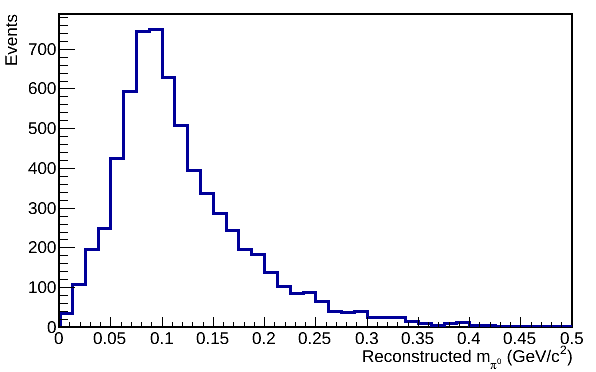
\includegraphics[width=0.8\textwidth]{pizeromass}
\end{cdrfigure}
\fixme{add figure; establish reference to calibration section; figure could also be at home in calibration section instead.}


\paragraph{PANDORA}
The reconstruction framework PANDORA~\cite{pandora} also works by
building up a three-dimensional picture from two-dimensional
reconstructed objects.  PANDORA is a flexible framework developed for
ILC detector simulation, and provides a convenient way to develop
algorithms for reconstructing particles.  In all, more than 80
algorithms, each targeting a specific topology, have been incorporated
into PANDORA to date.  Multiple passes through reconstructing the data
are possible.  Different criteria for clustering hits into tracks and
showers may be applied when seeking cosmic rays for removal rather than for
identifying signal events.  PANDORA proceeds by clustering hits in 2D,
reconstructing vertices in 3D, reconstructing tracks in 3D,
reconstructing showers in 3D, a mop-up step in 2D and 3D, followed by
full event building in 3D.

The performance metrics are efficiency, purity, and completeness.  The
efficiency of the algorithm is the fraction of true particles that
match reconstructed objects within the bounds of pre-specified
criteria, such as matching position and length and the type of object
expected.  The purity of the reconstructed object is the fraction of
hits (or charge) included in that object that truly came from the
matched particle divided by the total number of hits (or charge)
included in the reconstructed cluster.  The completeness is defined as
the number of true hits that are found in a cluster or track or shower
expressed as a fraction of total true hits in that object.  Plots of
the efficiency and completeness for muons in charged-current $\nu_{\mu}$
events in MicroBooNE are shown in Figure~\ref{fig:muonpandoraperf}.
The resolution of vertex-finding is shown in
Figure~\ref{fig:pandoraresolution}.
\fixme{Don't we have such a figure specifically for  protoDUNE ? If not, it should be a high priority task.}

\begin{cdrfigure}[Performance of PANDORA for muons in CC
  $\nu_mu$ events in MicroBooNE. ]{muonpandoraperf}{The performance of PANDORA for muons in charged-current
  $\nu_mu$ events in MicroBooNE. }
%\includegraphics[width=0.95\textwidth]{muonpandoraperf.png}\end{cdrfigure}
\end{cdrfigure}

\fixme{Include figure of PANDORA performance for muons.  Efficiency and
completeness (purity too if we can get the plot).}

\paragraph{PMA}
Another approach to 3D reconstruction in LArTPC detectors is called Projection Matching Algorithm
(PMA) ~\cite{pma_algorithm}. PMA was primarily developed as a technique of 3D reconstruction
of individual particle trajectories (trajectory fits) ~\cite{icarus3dreco}. Instead of
building up a 3D hypothesis from 2D clusters, it starts with the 3D hypothesis and compares
the 2D projection of predicted trajectory with the observed data. With such an approach
the associations between 2D planes on the level of individual hits can be avoided.
In consequence, the algorithm may deal with problematic cases, such as isochron tracks,
e.g. tracks with few-hits.

PMA can take as input the output from different pattern recognition algorithms, from
LineCluster ~\cite{linecluster} to WireCell (described below). As a result of 2D pattern
recognition performed independently in each 2D projection, particles may be broken
into several clusters, fractions of particles may be missing in individual projections
and clusters obtained from complementary projections are not guaranteed to cover corresponding
sections of trajectories. Such behavior is expected since ambiguous configurations of
trajectories can be resolved only if the information from multiple 2D projections is used.
PMA performs higher level pattern recognition using as input clustering information from all
projections in order to search for the best matching combinations of clusters. The algorithm
also attempts to correct hit to cluster assignments using properties of 3D reconstructed objects.

The 3D trajectory can be reconstructed using clusters from two projections while the distance of
the trajectory projection to data in the third plane is used to validate correct association of clusters.
This method is used to score 3D track candidates in the three-plane TPC configurations, like single-phase
DUNE and MicroBooNE detectors and prototypes. Clusters from all planes are used in this scenario in the
fine tuning of the selected candidates. In the two-plane configurations (dual-phase TPC detectors, single-phase
LArIAT and ArgoNeut detectors) the track candidates are scored by the value of its goodness of fit, which is
significantly decreased if the trajectory is being optimized to spuriously associated clusters.

PMA allows to build and optimize complex structures of 3D objects, i.e. multiple particle trajectories
interconnected with interaction vertices, relying on the same principle as for the single trajectory fit.
In this scenario the vertex position reconstruction employs the local information from several tracks
simultaneously, leading to an improved fit of each individual trajectory. The track-vertex structure
is constructed after the individual particle trajectories are reconstructed and their parts recorded
in different TPC volumes are associated and merged into single objects.
The reconstructed structure is described as a particle hierarchy using the LArSoft data structures
designed to save in the output file reconstructed objects and relations between these objects.

PMA has been used successfully to reconstruct simulated beam particles in
ProtoDUNE-SP. The spatial resolution of the interaction vertex with neutral pion
production, appearing in the positive pion 2 GeV/c sample, is shown in Figure ~\ref{fig:PMApioninteraction}
in order to illustrate the performance of the entire reconstruction chain. The spatial resolution
of 0.6 cm was found in this study. Similar resolution was obtained also for the reconstruction
of inelastic interaction vertices in the proton 2 GeV/c sample. A study of the reconstruction performance
specifically for particles with orientations as those expected for beam particles was carried out as a check.
\fixme{A sentence on some known problems with specific directions would be useful to provide more background info for non-expert readers.}
% that it is not introducing major difficulties to the analysis. 
Example results are shown in
Figure~\ref{fig:PMAdirection}, showing the minimal resolution deterioration for the isochronous
tracks (and a larger dependence on the length of the reconstructed track). Figures ~\ref{fig:PMAproton2gevc}
and ~\ref{fig:PMAcosmics} show examples of reconstruction of a 2 GeV/c proton in the test beam and
cosmic muons, respectively.

%\fixme{Include figure of PMA's resolution on the entry point for charged
%particles See Robert's talk from the April collab meeting - DONE (plots are for the pi+ interactions
%where pi0 was produced, entry point is almost trivial and simulation does not include complications
%on the tpc edges, interactions inside tpc are at bit more realistically simulated)}

%\fixme{Include figure of PMA's direction on the direction for charged particles See Robert's talk from the April collab meeting - DONE}


\begin{cdrfigure}[Vertex resolution for
  inelastic interaction of charged $\pi$'s on Ar nuclei where a $\pi^0$ is produced]{PMApioninteraction}{Vertex position resolution in cm in $x$, $y$, and $z$ and 3D for the
  inelastic interaction of charged pions on liquid argon nuclei in events in which a $\pi^0$ is produced, in
  ProtoDUNE-SP, using the PMA algorithm.\fixme{increase size of stat box entries; if possible remove "temp" header}}
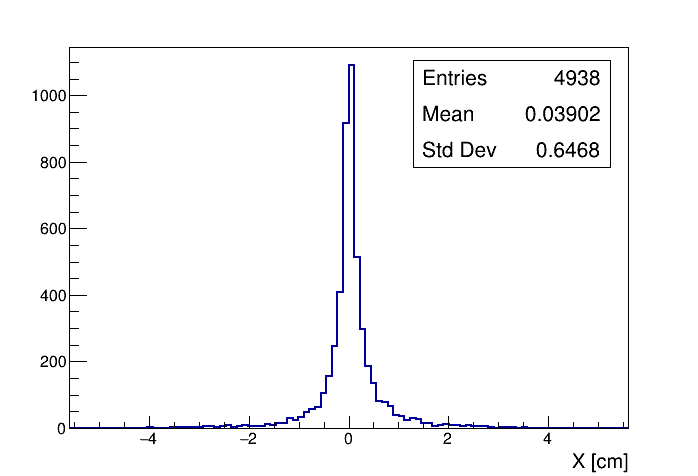
\includegraphics[width=0.45\textwidth]{pi0_vtx_dx.png}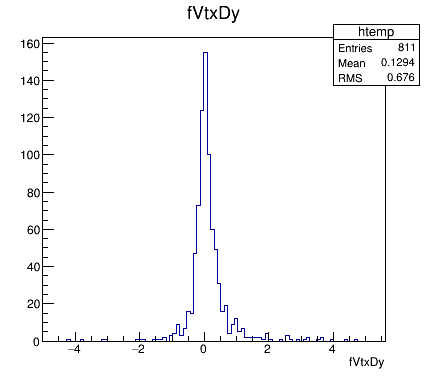
\includegraphics[width=0.45\textwidth]{figures/pi0_vtx_dy.png}
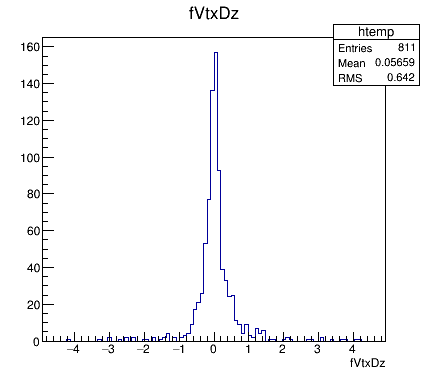
\includegraphics[width=0.45\textwidth]{pi0_vtx_dz.png}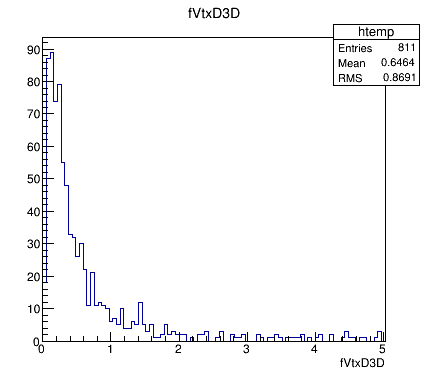
\includegraphics[width=0.45\textwidth]{figures/pi0_vtx3d.png}
\end{cdrfigure}

\begin{cdrfigure}[Primary beam particle direction resolution for protons 2GeV/c, as a function of true trajectory orientation in ZX plane (isochronous tracks are at 0 degree), ZY plane (horizontal tracks are at 0 degree) and as a function of the track length; trajectories reconstructed using gaushit, Line Cluster and PMA.]{PMAdirection}{Primary beam particle direction resolution for protons 2GeV/c, as a function of true trajectory orientation in ZX plane (isochronous tracks are at 0 degree), ZY plane (horizontal tracks are at 0 degree) and as a function of the track length; trajectories reconstructed using gaushit, Line Cluster and PMA. \fixme{need to increase axes label size; maybe draw equi-density lines in figures to help get the message across. }}
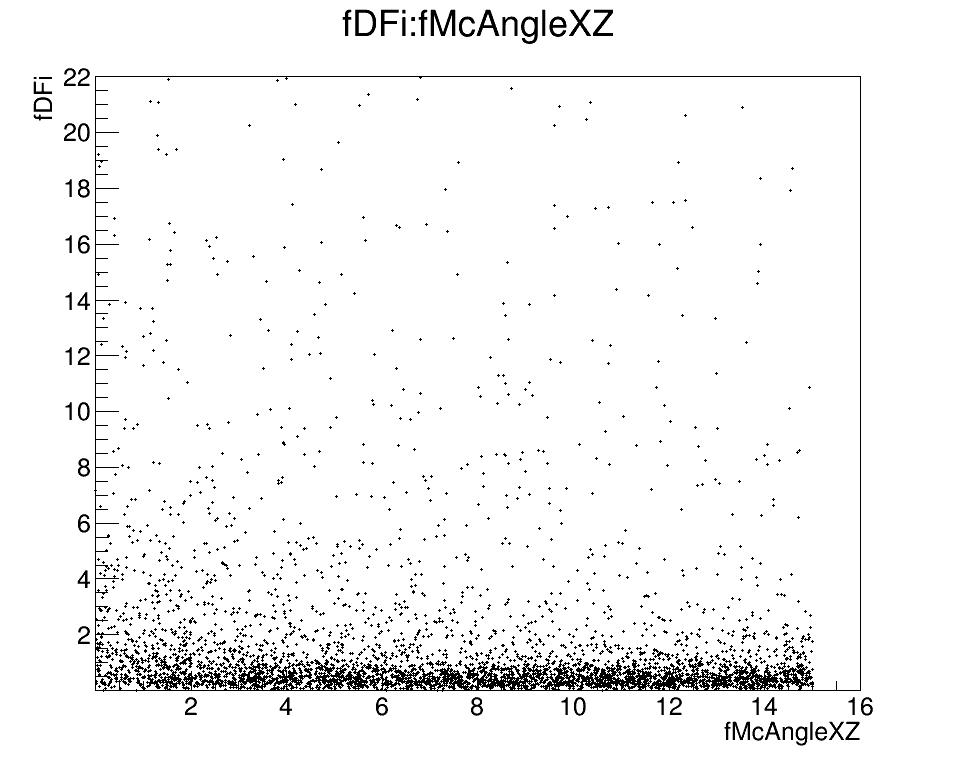
\includegraphics[width=0.3\textwidth]{figures/dFi-vs-beamXZ_primary_ptoton.png}
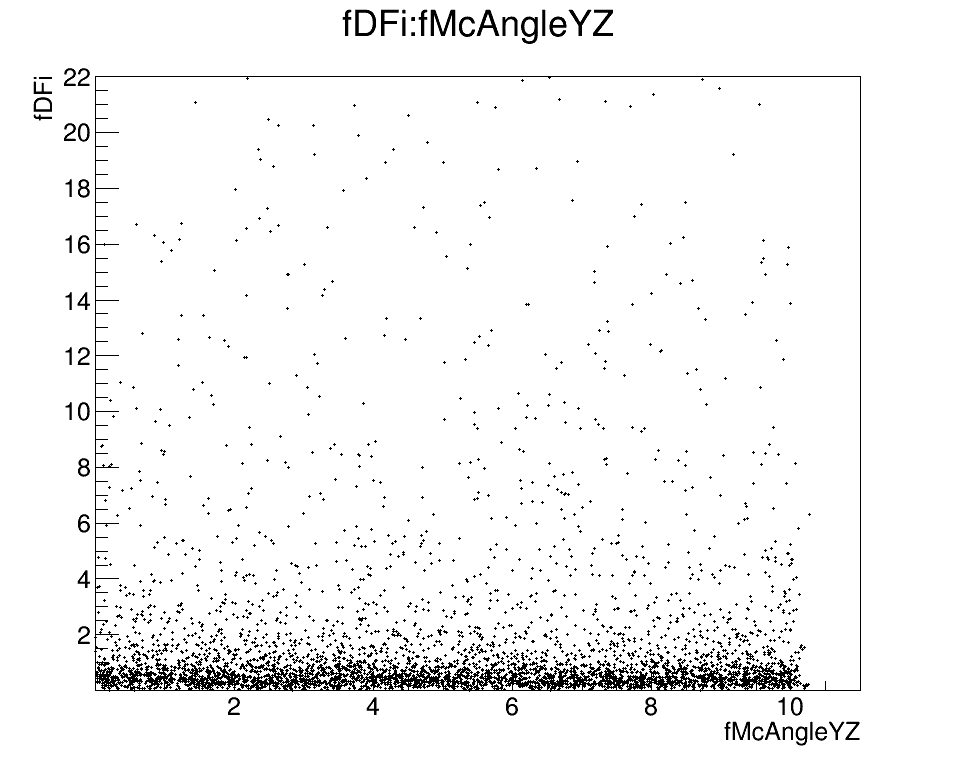
\includegraphics[width=0.3\textwidth]{figures/dFi-vs-beamYZ_primary_proton.png}
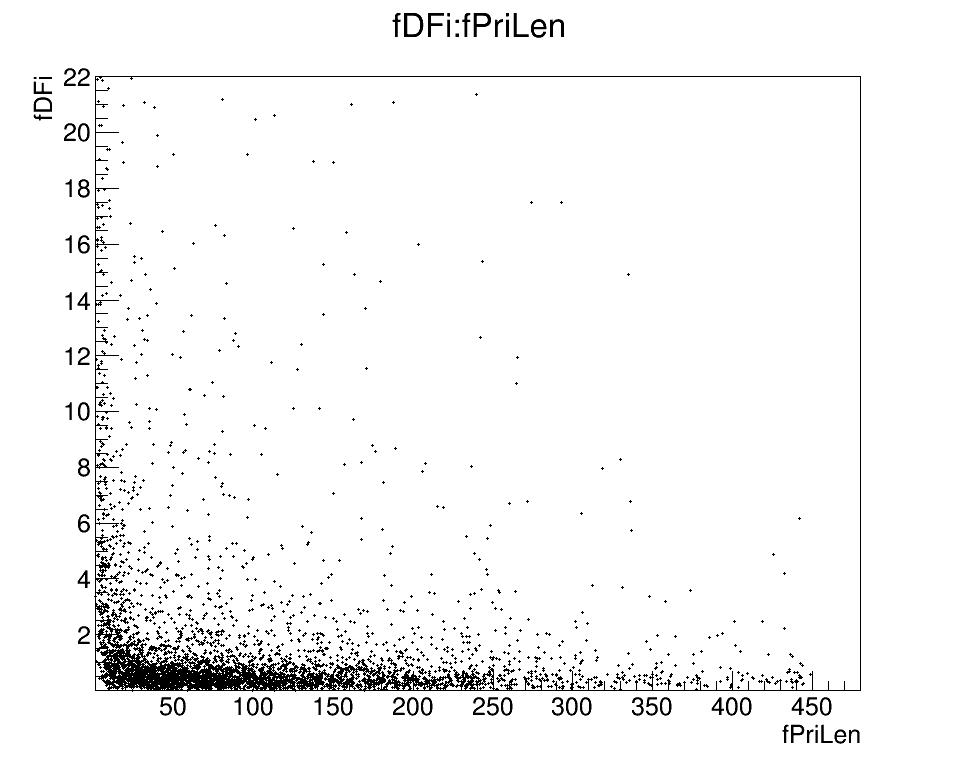
\includegraphics[width=0.3\textwidth]{figures/dFi-vs-TrkLen_primary_proton.png}
\end{cdrfigure}

\begin{cdrfigure}[Example of reconstructed event of simulated proton with initial momentum 2 GeV/c]{PMAproton2gevc}{Example of reconstructed event of simulated proton with initial momentum 2 GeV/c (reconstruction algorithms: gaushit, Line Cluster and PMA).}
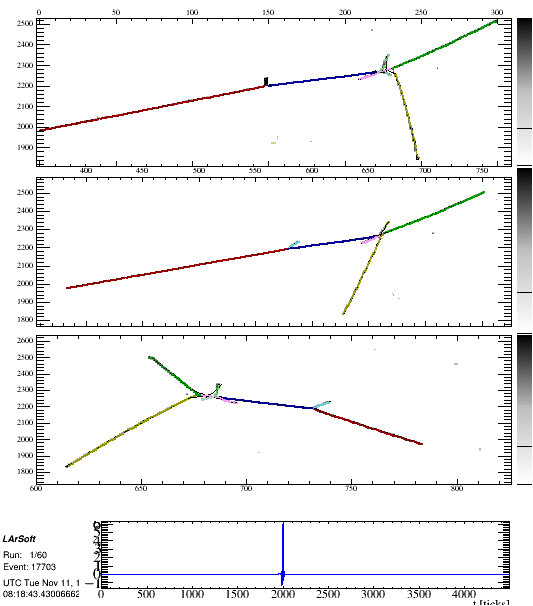
\includegraphics[width=0.45\textwidth]{figures/evdtwqproj117703.png}
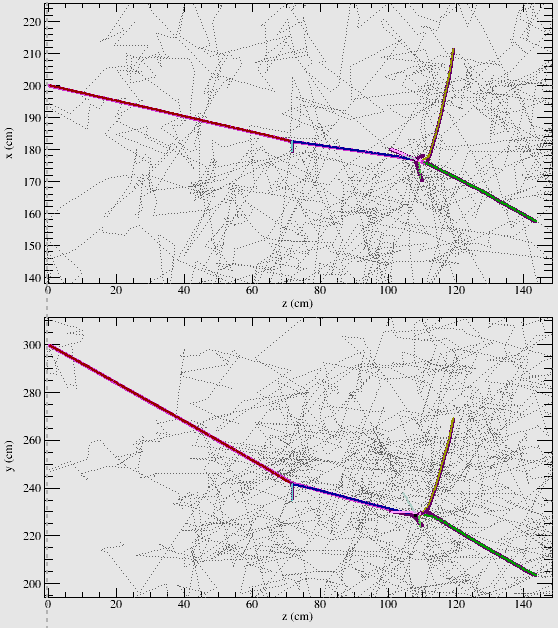
\includegraphics[width=0.45\textwidth]{figures/evdlarortho3d117703.png}
\end{cdrfigure}
\begin{cdrfigure}[Example of reconstructed cosmic muons in protoDUNE]{PMAcosmics}{Example of reconstructed cosmic muons using gaushit, Line Cluster and PMA.}
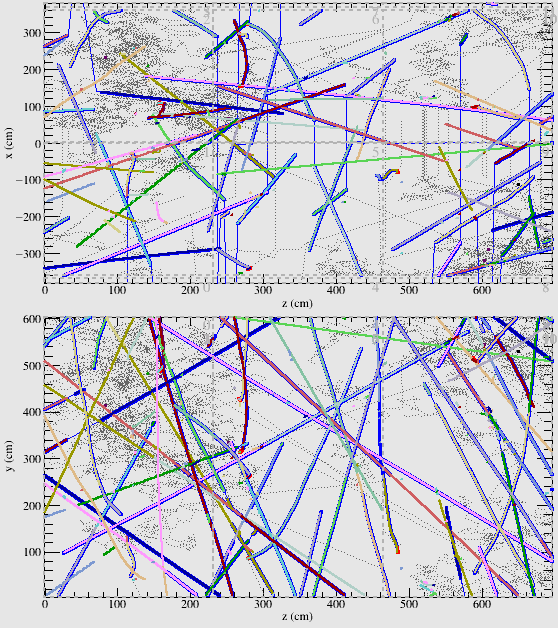
\includegraphics[width=0.45\textwidth]{figures/evdlarortho3d11302.png}
\end{cdrfigure}



%% Wire-Cell ... 
\paragraph{WireCell}
WireCell~\cite{wire-cell} adopts a very different approach from the 
fore-mentioned algorithms and is a new reconstruction method under development.
Instead of directly doing pattern recognition on each of the 2D views (drift 
time vs. wire number), the first step of the WireCell reconstruction is to 
perform 3D imaging with time, geometry, and charge information. The definition
of "Hit" is based on signal strength after charge extraction (described in 
Sec.~\ref{sec:tpc-signal-calibration}) in a 2 $\mu$s time slice. The usage of 
time information means that hits from different wire planes at different time 
slices cannot be associated. The usage of geometry information means that hits
from wires that are not crossing each other cannot be associated with each other. 
The usage of charge information means that hits from different wire planes
with different signal strengths are unlikely to be associated with each other. The 
usage of the charge information is quite unique for a LArTPC, as each of the 
wire planes in principle detects the same amount of the ionization electrons. 
Figure~\ref{fig:quality} shows an example of the performance of the WireCell 3D imaging. 
The large blue blob reflects the ambiguities due to wire readout for a track
traveling parallel to the wire plane (not necessary to the wire directly). A 3D web-based 
display can be found at \cite{ref:wirecell-3D}. 
For these types of events a group of wires from each 
wire plane fires simultaneously. Therefore, the time and geometry 
information will provide rather limited constraints on the hit associations.
%\fixme{Parallel to a wire in one of the planes implies that for the other two planes multiple wires should be crossed - so, why does geometry still provide limited information ??} 
The advantage of the WireCell approach is that it utilizes full TPC 
information. The requirement is i) hits arriving at different time slice cannot be
matched together, ii) hits from different wire planes arriving at the same time slice
cannot be matched together if the wires are not crossing at the same overlapping region, 
and iii) hits from different wire planes arriving at the same time slice and crossing
at the same overlapping region are unlikely to be matched if their charges are quite different. 
These strong requirements 
%\fixme{which requirements exactly ? spell out what these requirements are.}
on the time/geometry/charge information provides a natural way to suppress electronic noise.
The suppression of the electronic noise is at the cost of being more
sensitive to hit inefficiencies due to for example dead channels or improper signal processing.
%\fixme{What type of hit inefficiencies ??}
 Since the track and shower hypotheses
are not used, the 3D imaging works for any event topology. Once the 3D
images are reconstructed, 3D pattern recognition is needed to identify 
the content inside the image. Figure~\ref{fig:tracking2} shows the 
performance of the currently available 3D pattern recognition inside
WireCell. For the long track going close to parallel to the wire plane, the reconstructed
track shows a zig-zag behavior. This is due to the current lack of fine track fitting algorithm
that is expected to be added in the near future. 
%\fixme{maybe add a comment why the straight track was missed.}
Further developments of the WireCell pattern recognition 
are needed before meaningful physics quantities can be calculated.
%
%% Wire-Cell Imaging
\begin{cdrfigure}[Comparison of imaging recon
qualities with and without charge information]{quality}{Comparison of imaging reconstruction 
qualities with and without the charge information. }
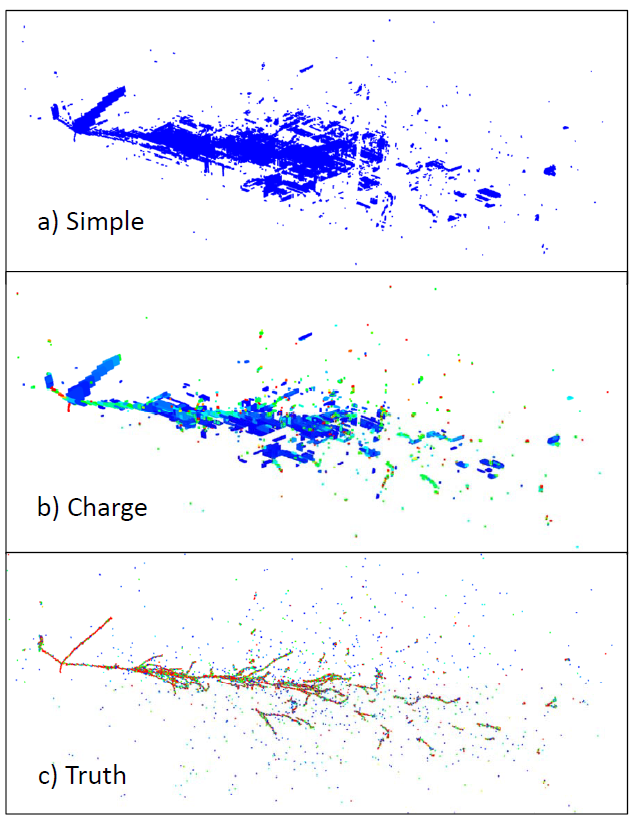
\includegraphics[width=0.5\textwidth]{quality.png}
\end{cdrfigure}
%
%
%% Wire-Cell 3D pattern recognition
\begin{cdrfigure}[Reconstructed image for one neutrino interaction event; comparison to MC]{tracking2}{The reconstructed image is shown 
on the left panel for one neutrino interaction event. The image 
was passed through the 3D pattern recognition program with tracks 
identified (middle panel). The identified pattern is compared 
with Monte-Carlo truth (right panel).}
 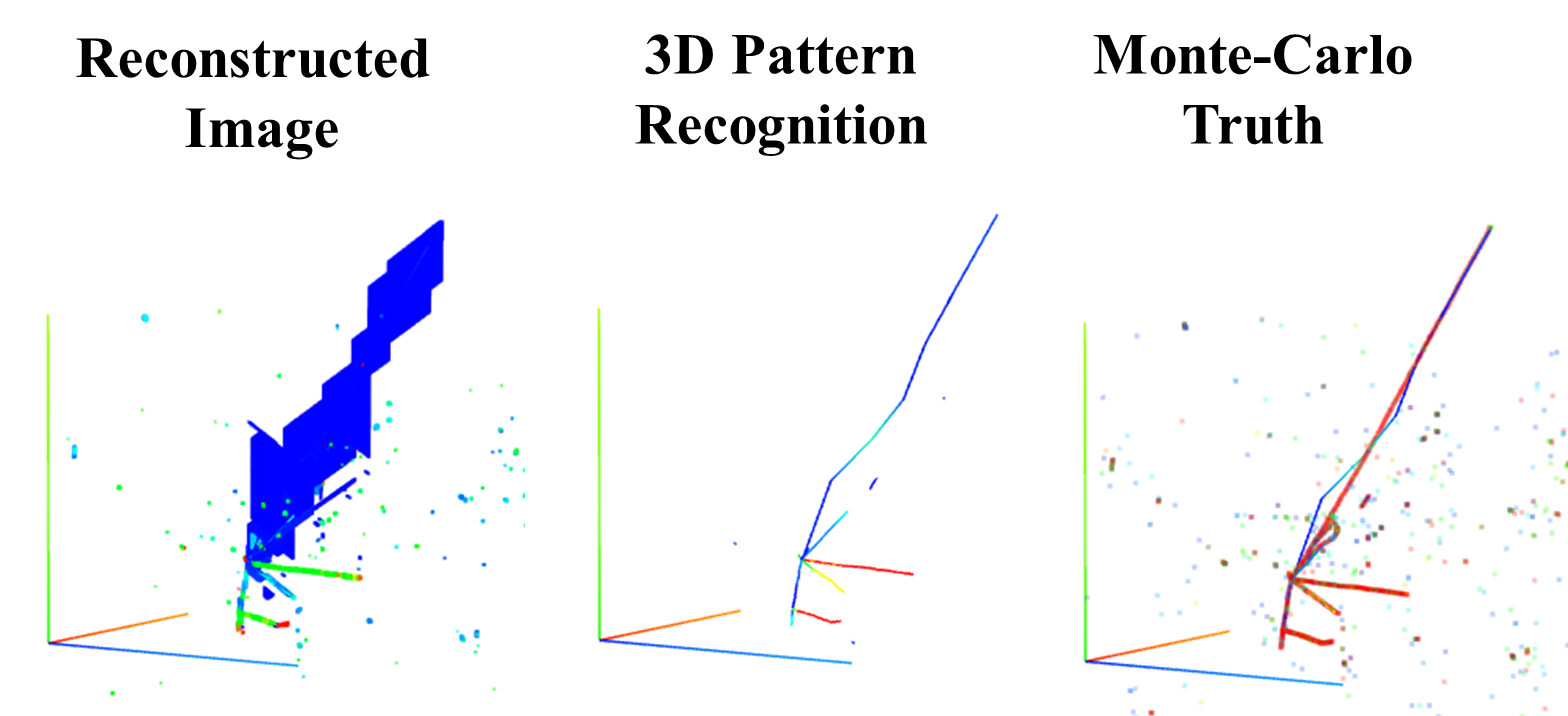
\includegraphics[width=0.9\textwidth]{Tracking_2.png}
\end{cdrfigure}


\fixme{A summary sentence or two describing the plans and goals for the reconstruction would be a nice round-out of this section. As is, the section ends rather abruptly.}
